\chapter{Umsetzung der Softwarearchitektur}
\label{cha:umsetzung}
\section{Softwaredesign auf den Mikrocontrollern}
\label{sec:Node-MCU}

\subsection{Softwarearchitektur und Designtools}

Die Softwarearchitektur auf den eingesetzten ESP8266-Mikrocontrollern wurde mit der Arduino-IDE angefertigt. Sie gliedert sich in zwei Hauptkomponenten:

\begin{itemize}
	\item \textbf{Setup-Funktion:} Verantwortlich für die Überprüfung der Kommunikationsfähigkeit der erstellten Kommunikations-Objekte.
	\item \textbf{Loop-Funktion:} Verwaltet den Zugriff auf den MQTT-Client, den PN532-Leser sowie das Auslesen und Schreiben der Speicherblöcke.
\end{itemize}


\subsection{Systemstart und Initialisierung}

Beim Systemstart werden zunächst globale Variablen und Objektinstanzen initialisiert, die für die spätere Kommunikation und Datenverarbeitung erforderlich sind [siehe \autoref{lst:init_globals}]. Dazu zählen:

\begin{itemize}
	\item Ein WiFi-Objekt, das die Netzwerkverbindung herstellt und damit die Grundlage für die MQTT-Kommunikation bildet.
	\item Ein SPI-Objekt, das die serielle Verbindung zum PN532-NFC-Sensor über das SPI-Protokoll ermöglicht.
\end{itemize}

Basierend auf diesen Kommunikationsschnittstellen werden zwei zentrale Objekte global angelegt:

\begin{itemize}
	\item Ein NFC-Objekt, das über das SPI-Objekt mit dem PN532-Sensor kommuniziert.
	\item Ein MQTT-Objekt, das über das WiFi-Objekt mit dem MQTT-Broker verbunden wird.
\end{itemize}

Zusätzlich werden globale Variablen definiert, die während der Laufzeit von verschiedenen Programmteilen gelesen und verändert werden können. Dazu gehören unter anderem:

\begin{itemize}
	\item die UID-Variable, welche die eindeutige Kennung des erfassten NFC-Tags speichert,
	\item sowie die io\_state-Variable, die den aktuellen Verarbeitungszustand an der Station eines Produkts repräsentiert.
\end{itemize}

\newpage

\begin{lstlisting}[language=C, caption={Initialisierung globaler Objekte und Variablen}, label={lst:init_globals}]
	// Globale Kommunikationsobjekte
	// SPI-connection
	PN532_SPI intf(SPI, PN532_SS);
	PN532 nfc = PN532(intf);
	// wifi and mqtt client 
	WiFiClient wifiClient;
	MqttClient mqttClient(wifiClient);
	
	// Globale Zustandsvariablen
	uint8_t uid_data[UID_LENGTH] = {0};
	uint8_t io_state[4] = {0};
\end{lstlisting}


In der Setup-Funktion, die einmalig beim Systemstart ausgeführt wird, werden die Verbindungen mithilfe der zuvor erstellten Objekte erstellt. Das Wifi-Objekt wird mit dem Netzwerk des Raspberry Pi verbunden. Dann kann über das MQTT-Objekt eine Verbindung zu dem Broker hergestellt werden. Mithilfe des NFC-Objekts wird überprüft ob die Verbindung zum PN532-Sensor über SPI hergestellt werden konnte. 

Das MQTT-Objekt wird außerdem dazu genutzt eine Callback-Funktion zu registrieren, mithilfe dieser der Informationsgehalt der empfangenen Nachrichten in die globale Zustands-Variable geschrieben wird. Zuletzt wird das Objekt genutzt, um ein Topic zu abonnieren. An der Werkerassistenzstation wird das Topic ''rfid/assembling\_mcu\_receive'' abonniert [siehe \autoref{lst:mqtt_sub}]. 

\begin{lstlisting}[language=C, caption={Abonnieren des MQTT-Topics in der Setup-Funktion}, label={lst:mqtt_sub}]
	// subscribe to a topic
	mqttClient.subscribe(topic_receive);
\end{lstlisting}

\subsection{Zustandsverarbeitung und Hauptschleife}

Die Hauptschleife folgt auf allen Mikrocontrollern der selben Logik wurde aber jeweils an die individuellen Anforderungen angepasst. Beispielsweise wird an der Werkerassistenzstation die UID eines Tags vergeben werden, falls es noch nicht geschehen ist. Ein Codeausschnitt dieser Station - explizit die Loop-Funktion - ist im Anhang festgehalten [siehe \autoref{lst:assembling_loop}].

Die Hauptschleife prüft kontinuierlich, ob ein NFC-Tag im Lesebereich erkannt wurde [siehe \autoref{fig:flowchart_mcu}]. Wird ein Tag erfasst, so wird die UID gelesen und die relevanten Speicherblöcke geschrieben [siehe \autoref{lst:writing_block}]. Wenn alle Informationen erfolgreich geschrieben wurden, wird eine Nachricht via MQTT mit den neuen Zuständen an den Broker gesendet. 

\begin{lstlisting}[language=C, caption = Funktion zum Schreiben einer Information auf einen Speicherblock am Beispiel der Werkerassistenzstation, label=lst:writing_block]
	success = nfc.mifareultralight_WritePage(ASSEMBLING_BLOCK, io_state_temp);
\end{lstlisting}

Für den Fall, dass eine Nachricht vom Broker empfangen wurde und ein Tag im Empfangsbereich ist, wird die erhaltene Information in den entsprechenden Speicherbereich geschrieben. Das erfordert jedoch, dass ein Tag an einer Station etwas länger verweilt. Diese Zeit wird festgehalten und wenn der Tag dann schließlich entfernt wird, wird eine erneute MQTT-Nachricht gesendet, die über die Weiterfahrt zur nächsten Station informiert. 

Diese Logik wird fortlaufend in einer Schleife durchlaufen.

\tikzstyle{startstop} = [rectangle, rounded corners, minimum width=3cm, minimum height=1cm,text centered, draw=black, fill=gray!20]
\tikzstyle{process} = [rectangle, minimum width=3cm, minimum height=1cm, text centered, draw=black, fill=blue!10]
\tikzstyle{decision} = [diamond, aspect=2, text centered, draw=black, fill=yellow!20, inner sep=1pt]
\tikzstyle{arrow} = [thick,->,>=stealth]


\begin{figure}[H]
	\centering
	\begin{tikzpicture}[node distance=1.5cm]
		
		% Nodes
		% start
		\node (start) [startstop] {Start Loop};
		\node (mqttpoll) [process, below of=start] {MQTT \texttt{poll()} aufrufen};
		\node (readtag) [decision, below of=mqttpoll, yshift=-0.5cm] {Tag erkannt?};
		\node (alreadywritten) [decision, below of=readtag, yshift=-1cm] {Tag bereits beschrieben?};
		\node (handlemsg) [decision, right of=alreadywritten, xshift=5cm] {MQTT-Nachricht erhalten?};
		
		% processes
		\node (writetag) [process, below of=alreadywritten, yshift=-1cm] {Zustand auf Tag schreiben};
		\node (readuid) [process, below of=writetag] {UID prüfen und ggf. zuweisen};
		\node (writetracking) [process, below of=readuid] {Tracking-Status auf Tag schreiben};
		\node (sendmqtt) [process, below of=writetracking] {MQTT-Nachricht an PI senden};
		
		% end
		\node (writetime) [process, below of=handlemsg, yshift=-2.5cm] {Tag-Zeit am Sensor festhalten};
		\node (tagdelay) [decision, below of=writetime, yshift=-1cm] {Länger als 2\,s im Feld?};
		\node (tagdetached) [decision, below of=tagdelay, yshift=-1cm] {Tag entfernt};
		\node (senddetach) [process, below of=tagdetached, yshift=-0.5cm] {MQTT: Statuswechsel an PI senden};
		
		\node (end) [startstop, left of=senddetach, xshift=-5cm] {Loop Ende / neuer Durchlauf};
		
		% Arrows
		% start
		\draw [arrow] (start) -- (mqttpoll);
		\draw [arrow] (mqttpoll) -- (readtag);
		\draw [arrow] (readtag) -- node[anchor= west] {ja} (alreadywritten);
		\draw [arrow] (readtag) -- node[anchor= west] {ja} (handlemsg);
		\draw [arrow] (readtag) -- ++(-3,0) |- node[anchor= north east] {nein} (start);
		\draw [arrow] (alreadywritten) -- node[anchor= east] {nein} (writetag);
		\draw [arrow] (handlemsg) -- node[anchor=south] {ja} (writetag);
		\draw [arrow] (alreadywritten.east) -- node[anchor=west] {ja} (writetime);
		\draw [arrow] (handlemsg) -- node[anchor=south] {nein} (writetime);
		
		% processes
		\draw [arrow] (writetag) -- (readuid);
		\draw [arrow] (readuid) -- (writetracking);
		\draw [arrow] (writetracking) -- (sendmqtt);
		\draw [arrow] (sendmqtt) -- (end);
		
		% dispatch decision
		\draw [arrow] (writetime) -- (tagdelay);
		\draw [arrow] (tagdelay) -- node[anchor=west] {ja} (tagdetached);
		\draw [arrow] (tagdelay) -- node[anchor=west] {nein} (end);
		\draw [arrow] (tagdetached) -- node[anchor=west] {ja} (senddetach);
		\draw [arrow] (tagdetached) -- node[anchor=west] {nein} (end);
		\draw [arrow] (senddetach) -- (end);
	\end{tikzpicture}
	\caption{Ablaufdiagramm der Hauptlogik auf dem Mikrocontroller}
	\label{fig:flowchart_mcu}
\end{figure}

\newpage

\subsection{Kommunikation über MQTT}

Die Kommunikation mit dem Dashboard erfolgt mithilfe eines Raspberry Pi über das MQTT-Protokoll. Jeder Mikrocontroller veröffentlicht Zustandsänderungen auf einem dedizierten Topic wie \texttt{rfid/shelf\_mcu\_send}. Die Daten werden im JSON-Format übertragen [siehe \autoref{lst:mqtt_json}].

\begin{lstlisting}[language=json, caption={Beispiel einer MQTT JSON Nachricht von der Werkerassistenzstation (0x04: zur Schraubstation, 1: iO) (siehe \autoref{tab:tracking_states})}, label={lst:mqtt_json}]
	{
		"uid": "AB CD EF 02",
		"tracking": "0x04",
		"state": "1"
	}
\end{lstlisting}

Werden Daten für ein abonniertes Topic empfangen, wird in die registrierte Callback Funktion [siehe \autoref{lst:mqtt_callback}] gesprungen und der erhaltene neue Zustand wird in die globale Zustands-Variable geschrieben. Zudem wird eine Variable gesetzt mit der dann in der Loop-Funktion erkannt wird, dass eine Nachricht empfangen wurde[siehe \autoref{fig:flowchart_mcu}]. Dadurch kann der neue Zustand, durch Zugriff auf die globale Variable in den Speicher des sich im Erkennungsbereich befindlichen NFC-Tags geschrieben werden. 

\begin{lstlisting}[language=C, caption={Registrierung des Callbacks in der Setup-Funktion}, label={lst:mqtt_callback}]
	// set the message receive callback
	mqttClient.onMessage(onMqttMessage);
\end{lstlisting}

\section{Visualisierung der Prozessdaten in Node-RED}
\label{sec:Node-Red}

\begin{figure}[H]
	\centering
	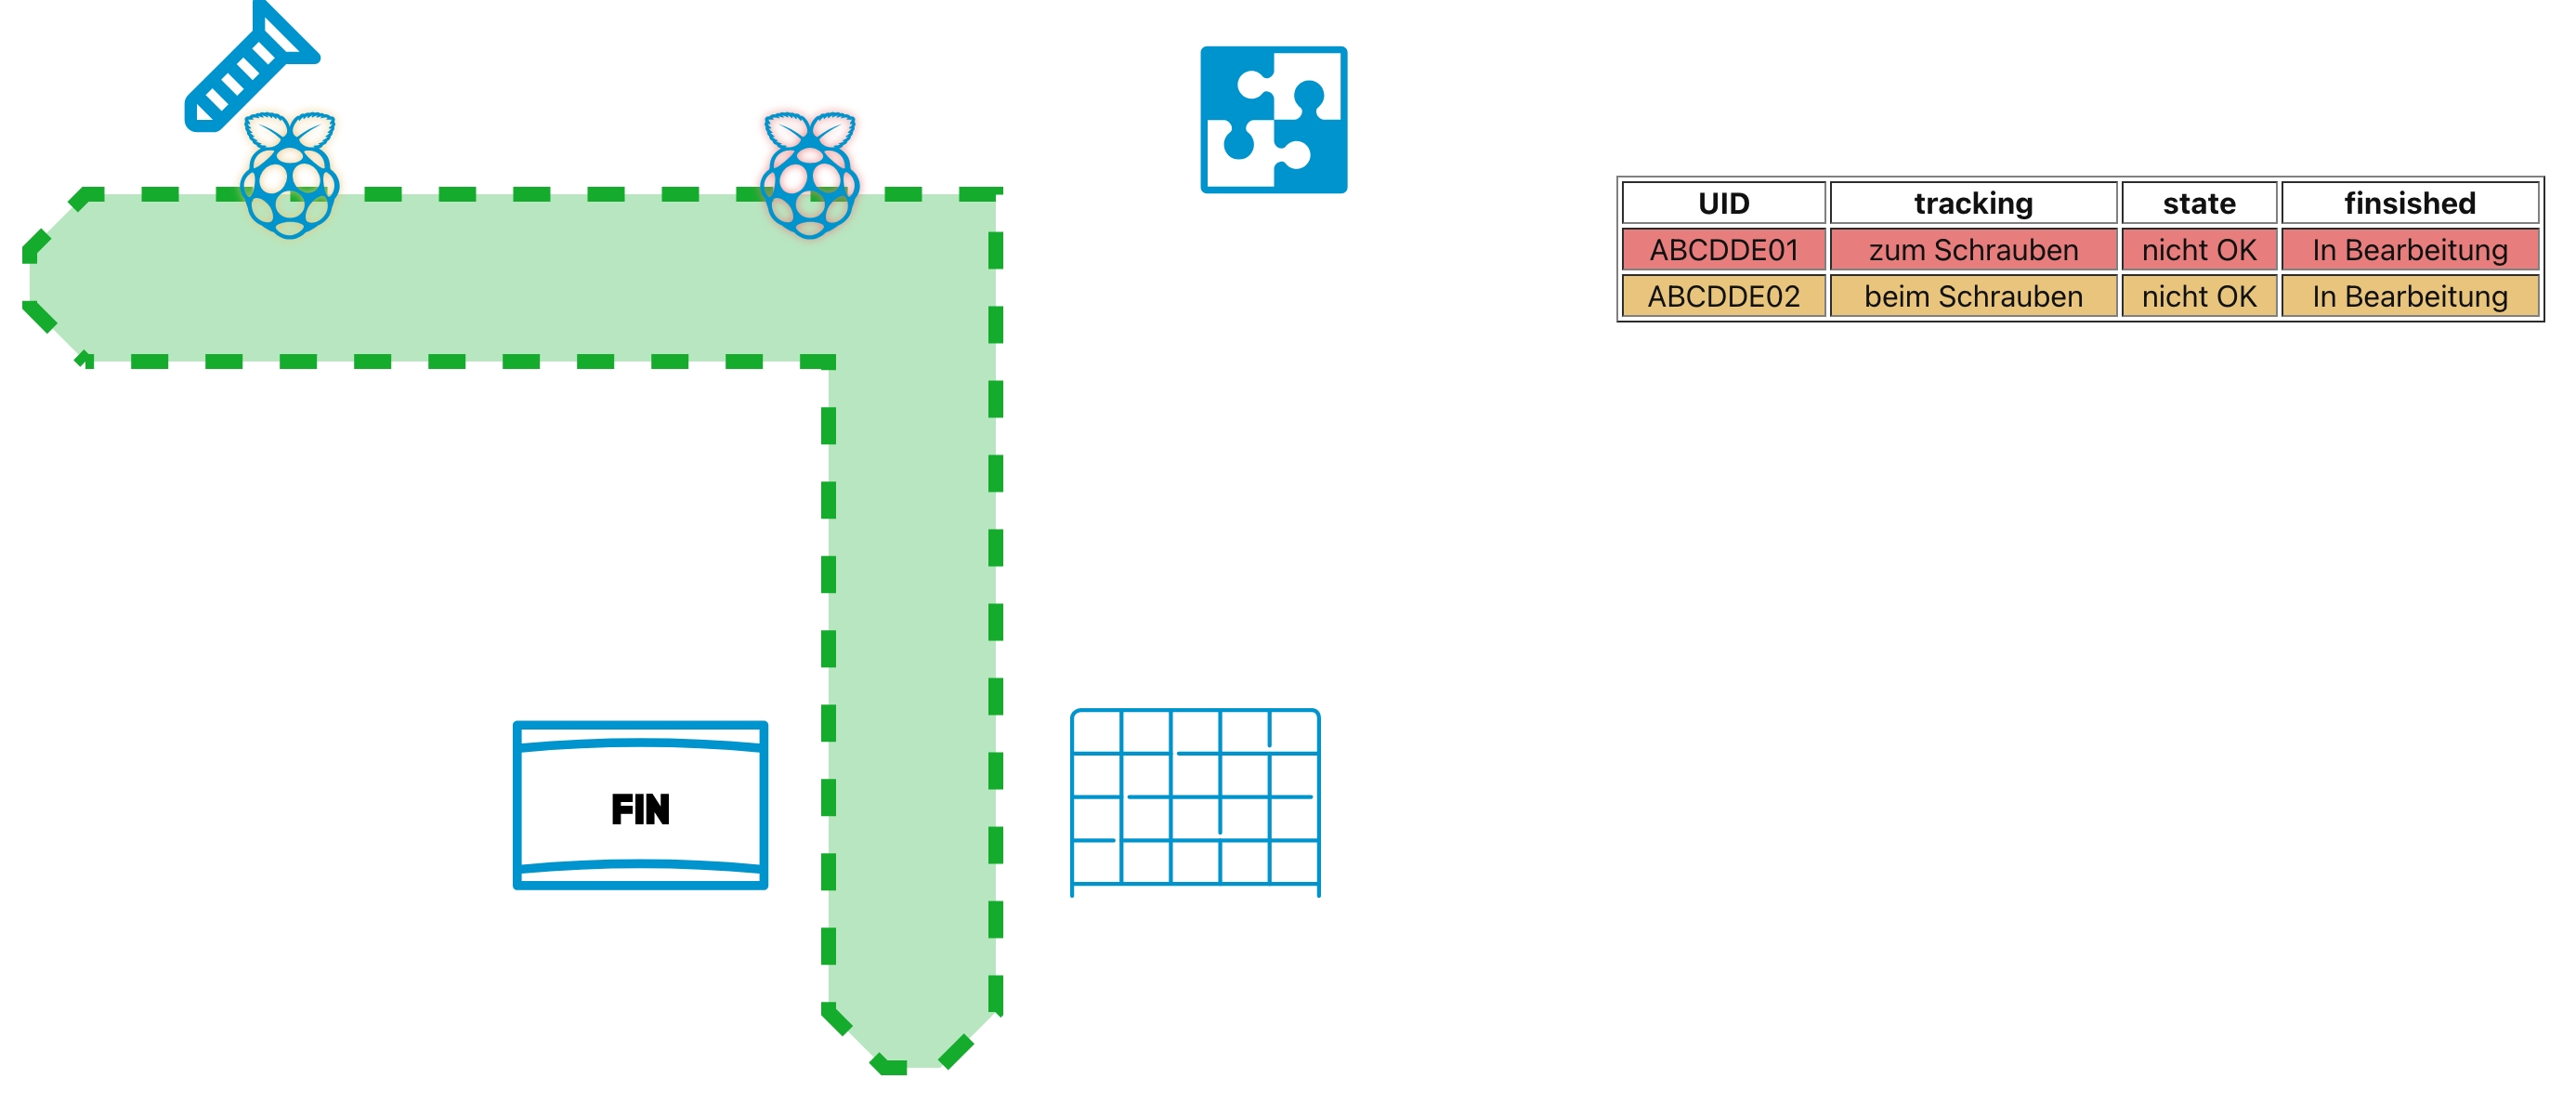
\includegraphics[width=0.8\textwidth]{images/node-red-band.jpeg}
	\caption{Node-RED-Dashboard des NFC-Tracking-Systems}
	\label{fig:dashboard}
\end{figure}

Zur Visualisierung der Produktpositionen und -zustände innerhalb des Bandumlaufsystems wurde ein interaktives Dashboard mit Node-RED implementiert (siehe \autoref{fig:dashboard}). Dieses Dashboard stellt die vier Stationen geometrisch entsprechend ihrer Anordnung in der Lernfabrik dar. Produkte werden symbolisch als Raspberry-Pi-Icons dargestellt und entlang des virtuellen Förderbands basierend auf ihrem erfassten Tracking-Zustand positioniert.

Die aktuelle Systemübersicht umfasst zwei Hauptkomponenten:
\begin{itemize}
	\item \textbf{Visuelle Darstellung des Förderbands:} Produkte bewegen sich entsprechend ihres Zustands zwischen den Stationen.
	\item \textbf{Tabelle mit Produktinformationen:} Für jedes Produkt wird eine eindeutige UID sowie der aktuelle Tracking-Zustand, der letzte Bearbeitungsstatus und ein Fertigstellungsindikator angezeigt. Die Zeilen sind farblich codiert, um die visuelle Unterscheidbarkeit der Produkte zu erhöhen.
\end{itemize}

\begin{figure}[H]
	\centering
	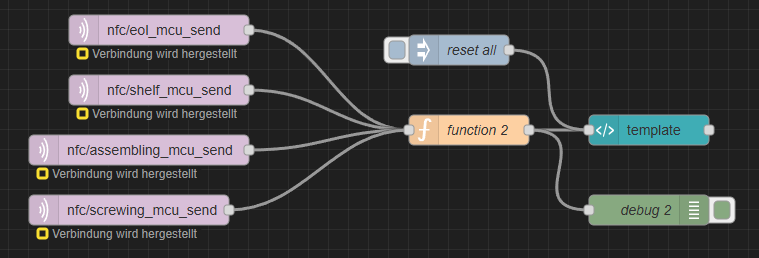
\includegraphics[width=0.8\textwidth]{images/node-red-flow-receive.png}
	\caption{Node-RED-Flow zum Empfang von Nachrichten}
	\label{fig:receive_nodes}
\end{figure}

Node-RED ermöglicht eine visuelle und modulare Abbildung der Prozesslogik. Die Empfangslogik ist in \autoref{fig:receive_nodes} dargestellt. Dabei werden vier verschiedene MQTT-Topics abonniert, über die jeweils eine der vier Stationen Nachrichten an das zentrale System sendet. Die empfangenen JSON-Daten werden über \texttt{MQTT-IN}-Nodes verarbeitet und anschließend von \texttt{Function}-Nodes analysiert. Die Logik in diesen Funktionsbausteinen umfasst:
\begin{itemize}
	\item Zuordnung der Nachricht zur entsprechenden Station
	\item Berechnung der exakten Position auf dem Dashboard
	\item Generierung einer individuellen Tabellenfarbe pro UID
\end{itemize}

Zusätzlich enthält der Flow einen Reset-Node zum Zurücksetzen des Dashboards sowie einen Debug-Node zur Laufzeitanalyse.

\begin{figure}[H]
	\centering
	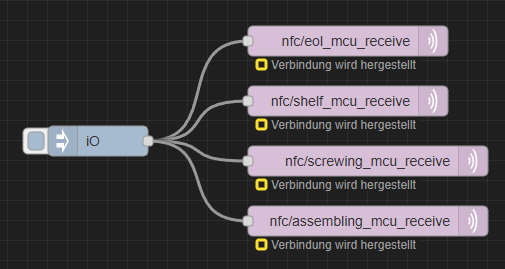
\includegraphics[width=0.8\textwidth]{images/node-red-flow-send.png}
	\caption{Node-RED-Flow zum Senden von Nachrichten an Stationen}
	\label{fig:send_nodes}
\end{figure}

Für Testzwecke wurde ein dedizierter Sende-Flow implementiert (\autoref{fig:send_nodes}). Dieser ermöglicht das manuelle Senden von Steuerinformationen an die Mikrocontroller an den Stationen über vier weitere MQTT-Topics. Diese haben dieselbe Namenskonvention wie die Empfangs-Topics, enthalten jedoch den Suffix \texttt{\_receive} anstelle von \texttt{\_send}. So kann eine einfache manuelle Steuerung einzelner Produktzustände direkt aus dem Dashboard heraus erfolgen.

\begin{table}[H]
	\centering
	\caption{MQTT-Topics}
	\label{tab:mqtt_topics}
	\begin{tabular}{|c|l|}
		\hline
		\textbf{Topic} & \textbf{Beschreibung} \\ \hline
		$rfid/eol\_mcu\_send$ & Datenübertragung von der EOL-Station zum Dashboard \\ 
		$rfid/shelf\_mcu\_send$ & Datenübertragung von der Lagerstation zum Dashboard \\ 
		$rfid/assembling\_mcu\_send$ & Datenübertragung von der Montage-Station zum Dashboard \\ 
		$rfid/screwing\_mcu\_send$ & Datenübertragung von der Schraubstation zum Dashboard \\ \hline
		$rfid/eol\_mcu\_receive$ & Steuerbefehl an die EoL-Station \\ 
		$rfid/shelf\_mcu\_receive$ & Steuerbefehl an die Lagerstation \\ 
		$rfid/assembling\_mcu\_receive$ & Steuerbefehl an die Montage-Station \\ 
		$rfid/screwing\_mcu\_receive$ & Steuerbefehl an die Schraubstation \\ \hline
	\end{tabular}
\end{table}


